\documentclass[../main.tex]{subfiles}

\begin{document}


\section{Confinamiento Magnético}
	\lhead[\thepage]{\thesection. Confinamiento Magnético}
	%--------------------------------------
	Dado que el plasma es un gas de iones y electrones, bajo las condiciones de temperatura y densidad correctas, es posible fusionar los núcleos que lo conforman. Hemos visto que, para que los núcleos de átomos ligeros puedan fusionarse, es necesario que cuenten con la energía suficiente para poder superar la repulsión eléctrica, además de otros factores. Para esto, es necesario confinar el plasma, y someterlo a altas temperaturas. Nunca se tendrá un confinamiento perfecto, y algunas partículas escaparán del plasma. Para mantener un plasma de fusión a altas temperaturas (temperaturas termonucleares) es necesario que el contacto del mismo, con las paredes del reactor sea mínimo, pues el plasma pierde energía y se enfría. Esto se logra usando campos magnéticos para confinarlo y que el contacto
    con el reactor sea casi nulo. Una partícula cargada con cierta velocidad $\vec v$ en una dirección, sometida a un campo magnético $\vec B$, experimentará un fuerza de Lorentz, la cual
    es perpendicular al plano formado por $\vec v$ y $\vec B$. La trayectoria descrita dependerá de que la partícula ingrese al campo magnético de manera perpendicular u oblicua.
    Dado que la fuerza de Lorentz siempre es perpendicular a la velocidad con que se mueve, está solo modifica la dirección de la trayectoria, mas no la rapidez. Dicho esto, en el caso general, cuando la partícula ingrese de manera oblicua, la componente perpendicular al campo $\vec B$ hará que la partícula describa un movimiento circular uniforme, mientras se mueve paralelamente a la dirección del campo, debido a la otra componente de la velocidad. Combinados ambos efectos, el movimiento total de la partícula será la de una hélice a lo largo de las líneas de campo, como se ilustra en la Figura (\ref{fig:trayectoria}), con radio de giro proporcional a la intensidad del campo magnético. \\
     
        \begin{SCfigure}
        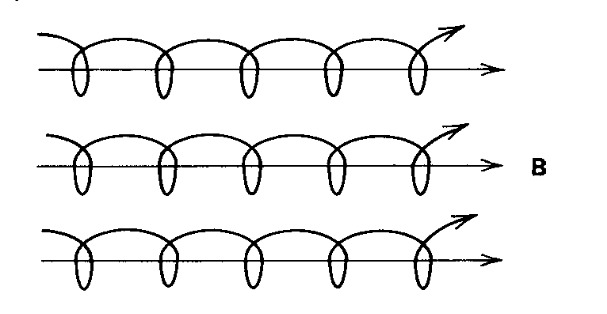
\includegraphics[width=8cm, height=4cm]{Particula.jpg}
        \caption{Trayectoria descrita por una partícula cargada en un campo magnético $\vec{B}$. Generalmente, las partículas seguirán las líneas de campo magnético \cite{stacey2010fusion}.}
        \label{fig:trayectoria}
        \end{SCfigure}

	    Como las partículas cargadas básicamente siguen las líneas de campo magnético, es necesario confinarlas dentro del reactor. Para eso, se distribuyen adecuadamente las fuentes de campo magnético. Un reactor Tokamak, tiene la forma de un donut, y consta de dos
        campos magnéticos combinados. Uno de estos, llamado campo toroidal, distribuye sus líneas a lo largo del eje interno del reactor. El segundo, llamado campo Poloidal, distribuye sus líneas magnéticas en  trayectorias cerradas en la sección transversal.  Combinados ambos, producen líneas de campo en forma de helicoide, y se logra confinar a las partículas
        dentro del reactor. Este concepto de reactor de fusión, fue concebido en la U.R.S.S a mediados de 1960 y es el que más interés 
        científico ha tenido. \\

        %\beginfigure{}

        \begin{figure}[h]
        \centering
        \includegraphics[width=0.6\textwidth]{Tokamak.jpg}
        \caption{Modelo básico de un reactor de fusión tipo Tokamak. Se observan las bobinas alrededor y a lo largo del reactor, que son las que producen el campo magnético toroidal al interior.}
        \end{figure}

        Otra manera de confinar las partículas, sin necesidad de confinar las líneas de campo magnético, es mediante el uso de pozos o espejos
        magnéticos. La manera en la que funciona este mecanismo, consiste básicamente en la conservación de la energía cinética y el momento
        magnético de la partícula. Dado que la fuerza de Lorentz actúa perpendicularmente a la dirección del movimiento, no hay trabajo realizado
        sobre la partícula. Además, el momento magnético también es una cantidad que se conserva. Entonces, se tiene que 
        \begin{align}
        &\frac{1}{2}m[v^2_{||}(s) + v^2_\perp(s)] = K, \\
        &\frac{1}{2}\frac{mv^2_\perp(s)}{B(s)} = \mu,
        \end{align}
        Donde $K$ y $\mu$ son constantes. Combinando ambas expresiones, tenemos que
        \begin{align}
            v^2_\perp(s) = \frac{2}{m}[K-\mu B(s)].
        \end{align}
        Podemos observar que el lado derecho de la ecuación podría desaparecer, si se tuviera un valor de $\mu$ lo suficientemente grande y, 
        en regiones donde el campo magnético sea intenso. Esto obligaría a la partícula a reflejarse en esas zonas, lo que haría que regrese,
        y permaneciera dentro de la cámara de reacción. Esto es lo que, idealmente sucedería. Sin embargo, hay regiones donde el campo magnético
        es bajo, y provoca ciertas inestabilidades que hacen que el plasma abandone esas regiones. Sin embargo, diversas configuraciones,
        como la de ``B mínimo", que básicamente son bobinas en forma de costuras de pelota de béisbol, compensan de alguna forma estos defectos.
        El espejo de Tándem, es un modelo de reactor que ubica esta configuración en cada extremo, lo que mantiene a las partículas cargadas en la
        región central.
        %--------------------------------------
    \section{Tokamak}
	\lhead[\thepage]{\thesection. Tokamak}

	    Un Tokamak posee la forma de un objeto geométrico llamado Toro, cuya superficie de revolución se obtiene rotando una circunferencia de 
        radio $r$ alrededor de un eje que se encuentra en el mismo plano de la circunferencia y a una distancia $R$ de su centro.

        \begin{figure}[h]
        \caption{Circunferencia de radio $r$}
        \centering
        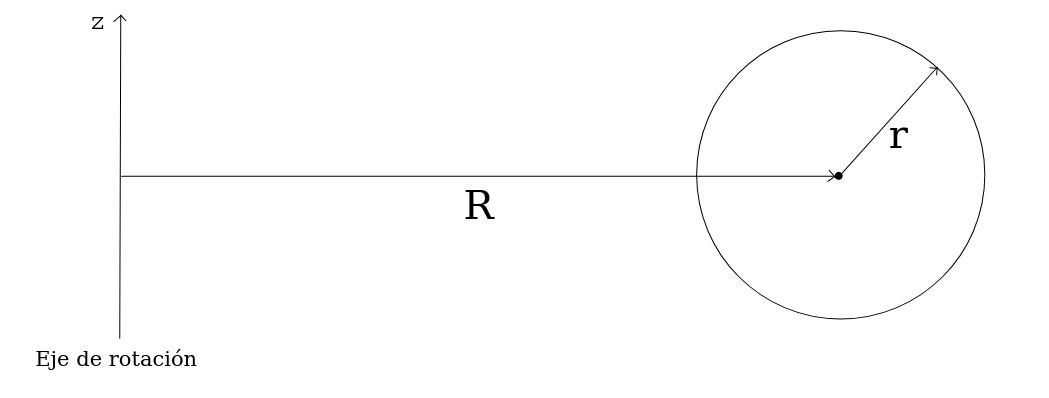
\includegraphics[width=0.7\textwidth]{Geometria_tokamak.jpg}
        \end{figure}

        Para especificar las coordenadas de cada punto en la superficie, y dentro del tokamak, usamos un conjunto nuevo de coordenadas
        $(\rho, \phi, \theta)$ los cuales están relacionados con las coordenadas cartesianas de la siguiente manera:

        \begin{align}
            &x = \left( R  + \rho\cos\theta \right)\cos\phi \\
            &y = s_{\phi} \left( R  + \rho\cos\theta \right)\sin\phi \\
            &z = s_{\theta} \sin\theta
        \end{align}

        Donde $0 \leq \rho \leq r$, $0 \leq \theta \leq 2\pi$, $0 \leq \phi \leq 2\pi$, y $s_{\phi} = \pm 1$, $s_{\theta} = \pm 1$ \\

        Suponiendo que, la circunferencia rota alrededor del eje Z, y el segmento de longitud $R$ se encuentra en el eje X, $\phi$ será 
        el ángulo barrido por $R$ en el plano XY, mientras que $\theta$ es el ángulo formado entre la coordenada $\rho$ de la circunferencia
        y el eje positivo X (o el segmento $R$). Los valores para $s_{\phi}$ y $s_{\theta}$ dependen de qué orientación se definirá para 
        el sistema, como se muestra en la Figura 3.4, donde se escogieron $s_{\phi} = s_{\theta} = 1$ \\ 

        \begin{figure}[h]
        \centering
        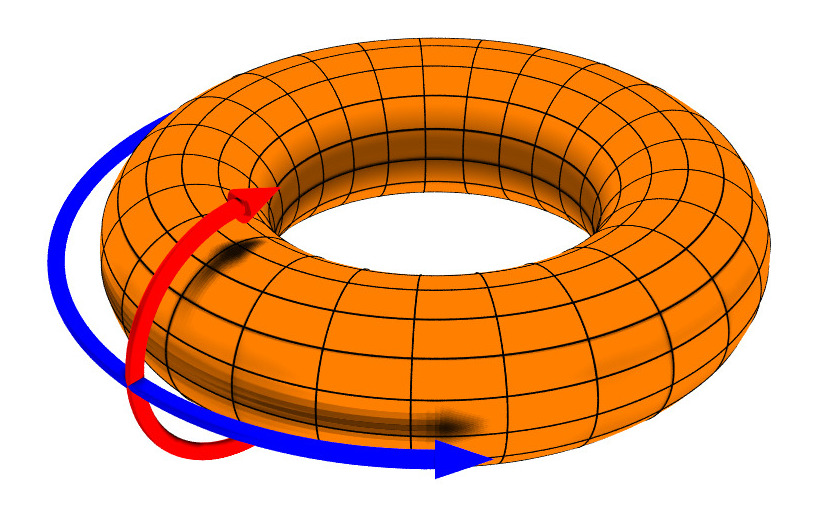
\includegraphics[width=0.5\textwidth]{Orientacion_tokamak.jpg}
        \caption{Vista geométrica de un tokamak, y las direcciones poloidal (rojo) y torodidal (azul).}
        \end{figure}

        La flecha azul indica la dirección toroidal, mientras que la flecha roja indica la dirección poloidal. Este nuevo sistema coordenado permitirá orientar ciertos campos magnéticos para confinar el plasma dentro del reactor, y estudiarlos mejor. Además, como ya se mencionó, Las partículas cargadas que poseen cierta velocidad $\vec v$, experimentan una fuerza si se encuentran bajo un campo magnético $\vec B$, de tal forma que
        \begin{align}
            \vec F_{\vec B} = q\left( \vec v \times \vec B \right).
        \end{align}
        Si además tenemos un campo eléctrico $\vec E$, la fuerza sobre la partícula cargada será
        \begin{align}
            \vec F_L = q\left( \vec v \times \vec B + \vec E \right),
        \end{align}
        donde $\vec F_L$ es la Fuerza de Lorentz. Aprovechando la influencia que tienen los campos magnéticos en la dinámica de las partículas cargadas, se describen dos disposiciones
        de campo magnético para un Tokamak. Por un lado, las líneas de campo magnético toroidal $\vec{B}_{Tor}$, se orientan a lo largo de la dirección toroidal del tokamak. Son generadas por
        bobinas dispuestas a lo largo del mismo, y la corriente que circula a través de ellas genera el campo. Por otro lado, en el campo magnético poloidal, las líneas de campo son circunferencias que se encuentran en la sección transversal del tokamak, y son producidas por corrientes eléctricas dentro del plasma, generadas por transformadores o bobinas exteriores al reactor. Este campo sirve para compensar la fuerza producida por la no uniformidad del campo toroidal, que hace que las partículas se dirijan radial mente hacia afuera del reactor. Para tener una idea, el campo magnético de la tierra en la superficie es de aproximadamente $\mathrm{45 \ \mu T}$. Si lo comparamos con el campo magnético toroidal del
        reactor PLT (Princeton Large Torus - 1975), donde $\mathrm{ B_{PLT}  = 1.6 \ T}$, tenemos de (\ref{equ_Bplt_Bt}), que el campo magnético toroidal del reactor PLT es más de 30 000 veces el campo magnético de la superficie terrestre
        \begin{align} \label{equ_Bplt_Bt}
            \frac{\left| \vec B_{PLT} \right| }{\left|  \vec B_{T} \right|} = \frac{1.6 \ T}{45 \ \mu T} \approx 3.6 \cdot 10^4.
        \end{align}
        
        \begin{SCfigure} 
        \caption{En la parte superior, tenemos la configuración de las bobinas responsables del campo magnético toroidal, en donde una corriente eléctrica fluye a través de estás. De igual forma, se induce una corriente interna dentro del plasma, lo que genera un campo adicional en la dirección poloidal, como se observa en el medio. La superposición de los dos campos, da como resultado que las líneas magnéticas se retuerzan y formen helicoides, como en la parte inferior.}
        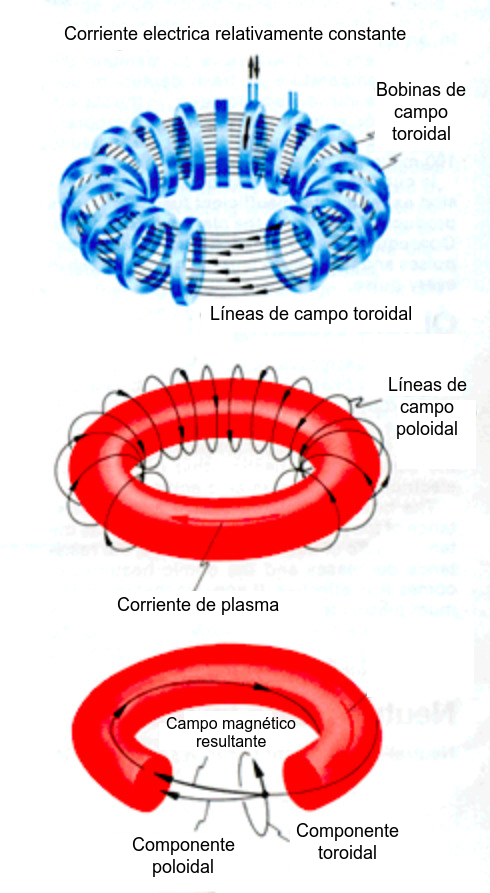
\includegraphics[width=0.385\textwidth]{Images/camp_toroidal_poloidal.jpg}
        \label{fig:lineas_magneticas_tor_pol}
        \end{SCfigure}
        
	    Dado que tenemos dos disposiciones de campo magnético dentro de un tokamak, estos se superponen para poder formar un campo magnético 
        $\vec B$ resultante. Este campo es helicoidal y cada línea se encuentra en una determinada superficie, dentro de un conjunto anidado
        de superficies toroidales. Para tener en cuenta, el campo magnético $\vec B_{Pol}$ es menor que $\vec B_{Tor}$. Las líneas helicoidales del campo magnético
        resultante (Figura \ref{fig:lineas_magneticas_tor_pol}), tienden a completar un recorrido poloidal después de algunos recorridos toroidales completos. Por lo general, estas líneas
        no se cierran a sí mismas, por lo que mapean toda una superficie de flujo magnético. Para conocer el número de recorridos 
        toroidales de una línea magnética, al completar un recorrido poloidal, desdoblamos el tokamak y adoptamos una figura cilíndrica de  
        longitud aproximada $2\pi R$, cuyo radio es igual a la de la sección transversal del tokamak $a$ (Figura \ref{fig:superficie_magnetica}). \\

    \begin{figure}[hbtp]
        %\centering
        \subfigure[]{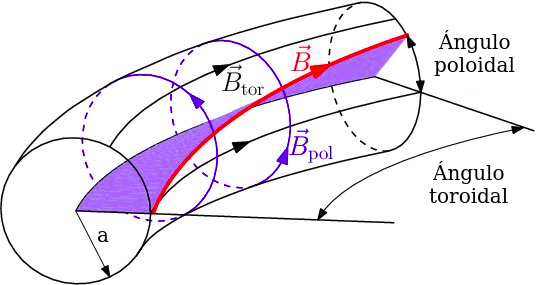
\includegraphics[width=8cm,height=5cm]{Images/Angulos_toroidal_poloidal.jpg}}
        \subfigure[]{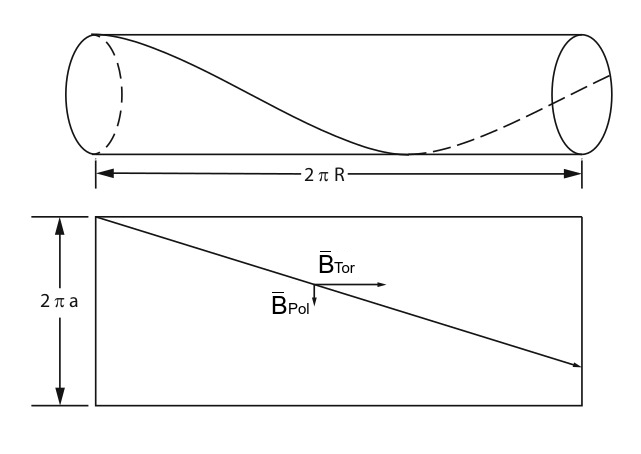
\includegraphics[width=8cm, height=5cm]{Images/Safety_factor.jpg}}
        \caption{a) Se puede observar una superficie de flujo magnético, en donde yacen las líneas del campo magnético resultante $\vec{B}_{Tor} + \vec{B}_{Pol} = \vec B$. b) Aproximación cilíndrica de un tokamak. El radio del toro es igual a R, mientras que el radio de la sección es transversal es $a$.} \label{fig:superficie_magnetica}
    \end{figure}
    
    Definimos entonces el factor de seguridad $q$, como el número de recorridos toroidales requeridos, para completar un recorrido poloidal de una línea magnética, donde se cumple que
    \begin{align}
        q = \frac{a}{R}\frac{\vec{B}_{Tor}}{\vec{B}_{Pol}}.
    \end{align}
    El factor nos da una idea de qué plasmas son sensibles a ciertas inestabilidades, como la inestabilidad de torsión, la que hace que el plasma tienda a deformarse y escapar rápidamente hacia las paredes del reactor. Para que esto no suceda, se debe cumplir que $q > 2$ \cite{morse2018fusion}. 
	    
	\section{Criterio de Lawson}
	\lhead[\thepage]{\thesection. Criterio de Lawson}

        En reactor de fusión tenemos mucha energía implicada. Ya sea la proporcionada para iniciar y/o mantener el proceso de fusión, o la producida durante las reacciones. Podemos entender el proceso dinámico de la energía que interviene, y el balance de energía, describiendo tres tipos de energías involucradas.
        De ahora en adelante se tomará de referencia a la energía por unidad de volumen y por unidad de tiempo $P$, pero solo la llamaremos energía a efectos prácticos. Tenemos entonces

        \begin{itemize}

            \item $P_{in}$: Energía suministrada al sistema 
            \item $P_{f}$: Energía producida por el sistema 
            \item $P_{out}$: Energía perdida por el sistema 

        \end{itemize}

        Tenemos entonces que, $P_{in}$ es la energía externa que se suministra al sistema para poder llegar a las condiciones requeridas para la fusión. Sabemos que, para que
        dos núcleos ligeros se fusionen, es necesario acercarlos lo más posible, para que la interacción nuclear fuerte pueda vencer la repulsión eléctrica. Para esto, se calienta el plasma a temperaturas muy elevadas, lo que da a las partículas (electrones e iones) la energía necesaria para 
        acercarse y a la vez, colisionar con átomos neutros y mantener el estado ionizado. Por otra parte, la energía externa sirve básicamente, para calentar el plasma. Los mecanismos por los cuales se suministra energía pueden ser, por ejemplo, radiación electromagnética. Una vez se alcancen las condiciones adecuadas para la fusión, los núcleos reaccionarán, y en este proceso se libera energía, o $P_{out}$. Para este caso analizamos la reacción D-T
        \begin{align}                 \mathrm{\tensor[^2]{H}{}+\tensor[^3]{H}{} &\longrightarrow  \mathrm{\tensor[^4]{He}{}+\tensor[^1]{n}{}}}.
        \end{align}
        Un núcleo de deuterio consta de un protón y un neutrón, mientras que un núcleo de tritio posee un protón y dos neutrones. Al fusionarse, se
        forma Helio-5, pero dado que el elemento es inestable, se desintegra rápidamente en Helio-4 y un neutrón energético. La energía obtenida en esta reacción la poseen las partículas resultantes en forma de energía cinética. En total, se produce una energía de 
        17.59 MeV, de los cuales, el 80\% aproximadamente la posee el neutrón, mientras que el resto es para la partícula alfa (Helio-4). Esto dificulta que el plasma pueda mantenerse por su propia energía producida, debido a que la mayor parte de la energía la tiene el neutrón.
        Como sabemos, esta partícula es neutra, por lo que no puede ser confinado por los campo magnéticos utilizados, y abandona rápidamente el  plasma para terminar en las paredes del reactor. Por otra parte la partícula alfa si posee carga eléctrica, por lo que se pueden usar los campos magnéticos para mantenerla dentro y así transfiera su energía al plasma. \\

        En el reactor se tendrán algunas perdidas de energía por la fuga del material, es decir, algunas partículas escaparán del plasma y esto disminuirá
        en parte la energía contenida. Además, también se tienen perdidas por radiación. Con esto podemos establecer una especie de balance de energía de un reactor de fusión con plasmas termonucleares

        \begin{align}
            W = P_{in} + P_f - P_{out},
        \end{align}
        donde $W$ es la energía neta. Se cumple entonces que
        \begin{itemize}

                 \item $W > 0$: El plasma gana energía para calentarse
                 \item $W < 0$: El plasma pierde energía y se enfría
                 \item $W = 0$: El plasma entra en un estado estacionario

        \end{itemize}
        Además, se define el tiempo de confinamiento $\tau_E$, como el tiempo que le tomaría al plasma apagarse o, vaciar su energía una vez que se dejara de suministrarla. Dado que $P_{out}$ es 
        la energía que va perdiendo el plasma, tendríamos que
        \begin{equation} \label{E_term}
            E_{term} = P_{out}\tau_E,
        \end{equation}
        Donde $E_{term}$ es la energía perdida por unidad de volumen. Dado que la energía de fusión es, principalmente, la energía que portan las partículas alfa, se tratará de generar la mayor cantidad de reacciones para que el plasma se auto sustentable energética mente. Esto significa que el plasma pueda mantener su temperatura y no se enfríe. Debido a que tenemos pérdidas de energías por distintos factores, inicialmente el plasma no podrá sostenerse por sí mismo, por lo que se
        tendrá que suministrar energía externa para mantener y aumentar el numero de reacciones. El cociente de la energía de fusión y la energía 
        suministrada es a lo que llamamos factor de amplificación Q, y se define como
        \begin{align} \label{Q}
            Q = \frac{P_f}{P_{in}}.
        \end{align}
        Idealmente, lo que se busca es que el plasma sea totalmente auto sustentable. Esto quiere decir que no se le suministre energía, lo que haría que Q fuese infinito, pues $P_{in}$ seria cero. Sin embargo, esto es imposible, puesto que siempre se tendrán perdidas de algún tipo. Entonces, el factor Q nos dice qué tan auto sustentable
        es nuestro plasma. Es por esto que se buscan valores altos para Q, y cuando es igual a 1, decimos que la energía de fusión es igual a la energía externa suministrada. Una mayor parte de la energía producida
        se usa para mantener el plasma. Cuando se genera suficiente energía para compensar las pérdidas, se puede dejar de suministrarla en mayor grado. Decimos entonces que el plasma ha entrado en ignición, por lo que
        \begin{align}
            Q \approx \infty.
        \end{align}

        Llegado a este punto, podemos definir, y deducir de manera básica, a lo que llamamos, el criterio de Lawson. Este criterio establece las condiciones mínimas para que un plasma pueda mantenerse, es decir, no se apague.
        Esto no significa que, el plasma será capaz de mantenerse a sí mismo mediante la energía producida, si no que el plasma no se apagará
        bajo las condiciones correctas, independientemente de como se mantenga.
        Para deducir las condiciones necesarias, consideramos un plasma formado por deuterio y tritio (fusión D-T). Por la cuasi neutralidad
        del plasma, tendremos que las densidades de electrones e iones son iguales. También asumimos que las densidades de deuterio y tritio son
        las mismas, entonces
        \begin{align}
            &n_e = n_i = n_D + n_T = n_0, \label{dens_fusion} \\
            &n_D = n_T = \frac{n_0}{2}. \label{dens_iguales}
        \end{align}
    Planteamos la siguiente condición
        \begin{align}
            P_f + P_{in} \geq P_{out},
        \end{align}
    y usando las ecuaciones (\ref{E_term}) y (\ref{Q}), tenemos que
        \begin{align}
            &P_f + \frac{P_f}{Q} \geq \frac{E_{term}}{\tau_E}, \\
            &P_f \left(1+ \frac{1}{Q} \right) \geq \frac{E_{term}}{\tau_E}. \label{final_condicion}
        \end{align}
        Necesitamos conocer la potencia de fusión y la energía térmica perdida por unidad de volumen. Para hallar $P_f$, multiplicamos el número de reacciones por unidad de volumen y por segundo (\ref{equ5}), y multiplicarla por la energía de fusión liberada en cada reacción. Tomando en cuenta también (\ref{dens_iguales}
)
        \begin{align}
            &P_f = N_{reac}E_f, \\
            &P_f = n_Dn_T\bar{<\sigma v>}E_f, \\
          &P_f=\frac{n_0^2}{4}<\sigma v>E_f. \label{final_pf}
        \end{align}
        Para calcular $E_{term}$, consideramos para una partícula $j$ en equilibrio térmico

        \begin{equation} \label{energia_termica}
            E_j= \frac{3}{2}k_BT_j.
        \end{equation}
        Luego, en el equilibrio todas las partículas estarán a la misma temperatura $T$. Podemos entonces calcular la energía térmica del plasma que se perderá en el intervalo de tiempo $\tau_E$ por unidad de volumen, multiplicando la densidad total de partículas por (\ref{energia_termica})        \begin{align}
            &E_{term} = n_eE_e + n_iE_i, \\
            &E_{term}= \left( n_e + (n_D + n_T) \right)\frac{3}{2}k_BT, \\
            &E_{term} = 3n_0k_BT. \label{final_Eterm}
        \end{align}
    Finalmente, reempĺazamos (\ref{final_Eterm}) y(\ref{final_pf} en (\ref{final_condicion}) 
        \begin{align}
          &E_f\frac{n_0^2}{4}<\sigma v>\left( 1+\frac{1}{Q} \right) \geq \frac{3n_0k_BT}{\tau_E}, \\
          &n_0\tau_E \geq \frac{12k_BT}{E_f\left( 1+\frac{1}{Q} \right)<\sigma v>}.
        \end{align}
        
        \begin{figure}[h]
        \centering
        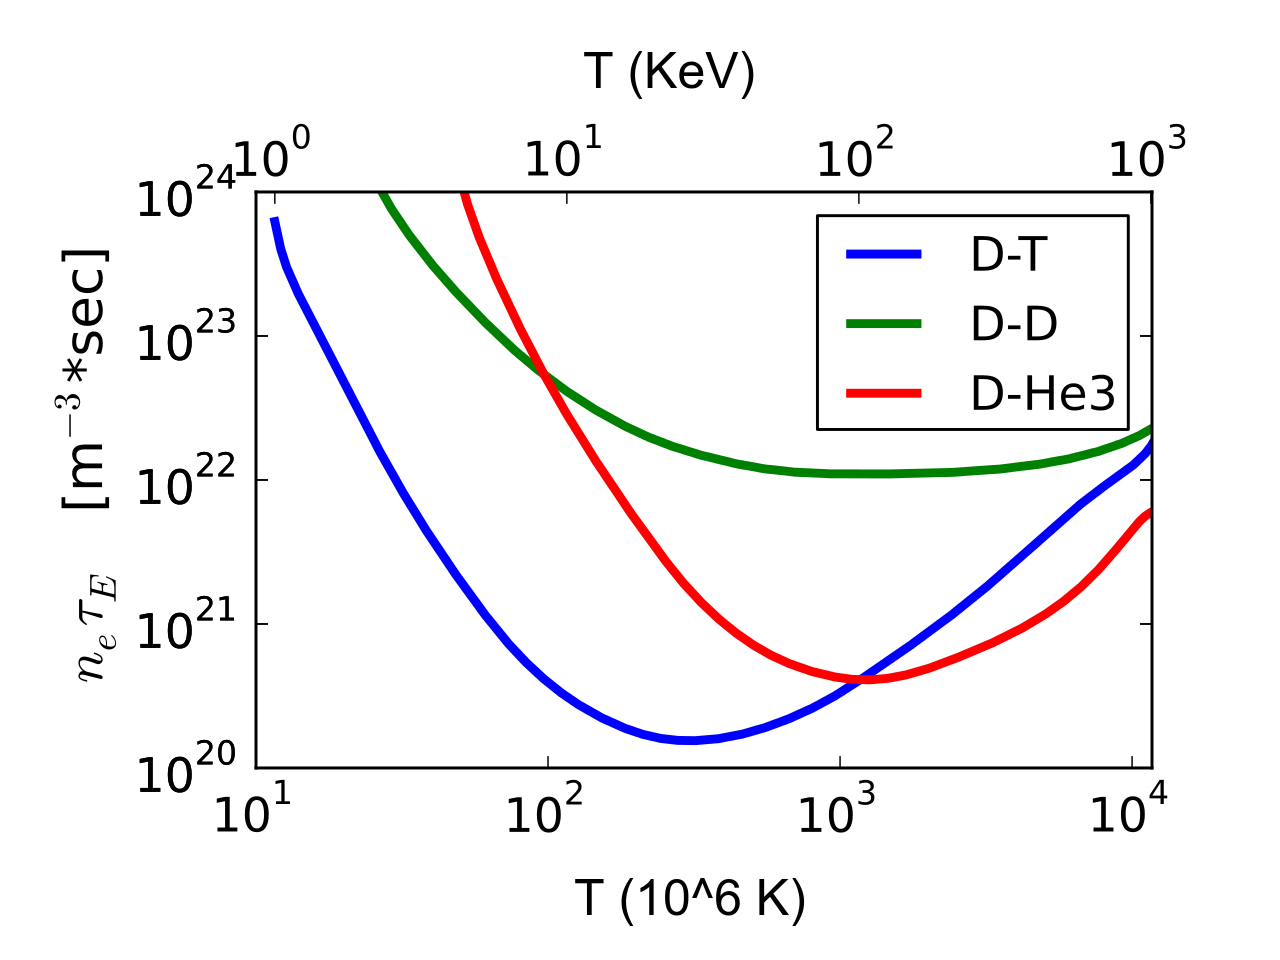
\includegraphics[width=0.8\textwidth]{Images/lawson.jpg}
        \caption{Comparación de los valores mínimos para el criterio de Lawson, en las reacciones de fusión D-T, D-D, y D-He3. Se observa que para la reacción D-T, se alcanza el mínimo a una menor temperatura.}
        \end{figure}
        
        Una forma alternativa de esta expresión implica a la temperatura también, y se le conoce como producto triple
        \begin{equation}
            n_0\tau_ET \geq \frac{12k_BT^2}{E_f\left( 1+\frac{1}{Q} \right)<\sigma v>}. \label{prodcuto_triple}
        \end{equation}
        La deducción anterior no tomo en cuenta los mecanismos específicos de perdida de energía, o los de auto calentamiento del plasma \cite{morse2018fusion}, pero aún se puede observar los aspectos generales del mismo. Para plasmas en estado de ignición, tomamos $Q$ muy grande, por lo que $1/Q$ es despreciable. Otro detalle a tomar en cuenta es que, la
        energía de fusión se debe a las partículas alfa que se producen durante la reacción. Líneas arriba se explico los motivos por los cuales
        no se toma en cuenta la energía debida a los neutrones. Para la reacción D-T, el valor mínimo de (\ref{prodcuto_triple}) para Q muy grande, ocurre cuando $T=14 \ \mathrm{KeV}$. A esta temperatura, también se puede considerar aproximadamente que $<\sigma v> = 1.1 \cdot 10^{-24}$ $T^2$ $\mathrm{m^3/s}$. Reemplazando estos valores en (\ref{prodcuto_triple}) y además $E_f = 3.5 \ \mathrm{MeV}$, tenemos que
        \begin{align}
            n_0\tau_ET \geq (n_0\tau_ET)_{min} \approx 3 \cdot 10^{21} \mathrm{KeV \frac{s}{m^3}}.
        \end{align}
        
	%---------------------------------------------
	
\end{document}


